\chapter{Requisitos y diseño}
\label{cap:introduccion}

%\chapterquote{}{}

\textcolor{red}{EN DESARROLLO: Éstá bastante desordenado, podríais indicarnos si está en el orden correcto, o qué podemos hacer para cohesionarlo. \\ El nombre es provisional, aunque suena bastante bien y ayuda a que no nos refiramos al proyecto como \textit{El proyecto} o \textit{Lo de los pictos}}



\begin{resumen}

	
	
	En este capítulo se explicará el proceso de creación de la aplicación PictUp. Ésta se trata de una aplicación web de creación y edición de tableros pictográficos interactivos. El capítulo se dividirá en las distintas fases del desarrollo: 1. Estudio de requisitos 
	
\end{resumen}

\label{cap1:sec:Motivacion}


\section{Introducción}

El propósito de la aplicación es la de solventar los problemas que otras aplicaciones traían y aunar las herramientas necesarias para facilitar la creación de tableros pictográficos. Otro objetivo es la de ofrecer interacción a los tableros, al estar éstos en un medio digital. 

PictUp está ideada para que sea útil tanto para padres o profesores que son los que crearán contenido pictográfico, como para las personas que puedan beneficiarse del uso de los tableros creados. Es por ello, que se pueden distinguir dos tipos de usuarios, el editor y el alumno. 

Las características que de estos han sido obtenidas del trabajo futuro de otros TFG, comentarios de los usuarios que utilizaban estas aplicaciones y sugerencias de los tutores.
\begin{itemize}
	\item Crear tableros con precisión.
	\item Utilizar fotografías como material.
	\item Agilizar el proceso buscar pictogramas que sean usados de manera recurrente.
	\item Añadir interacción a los tableros: Como hemos visto, muchas aplicaciones son rígidas, por lo que una vez creado el tablero no se puede hacer nada más, al añadir alguna clase de componente que permita no solo interactuar al alumno, sino que además el editor pueda dar distintos usos al componente para poder crear distintas actividades con el mismo elemento.
\end{itemize}






\section{Diseño de la aplicación}

Después de probar distintas tecnologías y estudiar la situación actual de los tablero pictográficos, se procedió a bocetar la idea de la aplicación y el formato de la interfaz. Al ser dos personas, se realizaron dos bocetos diferentes, de los cuales se obtuvieron los primeros componentes y asentaron las bases del proyecto.


\subsection{Prototipo realizado por Alfonso}

Teniendo en cuenta, los requisitos de los usuarios, las aplicaciones existentes y el trabajo futuro de desarrollado en trabajos similares, empezamos a bocetar una primera idea del proyecto.


En la Figura \ref{fig:loginalfonso} podemos ver el boceto de la pantalla de  inicio, la cual estaría compuesta por cuatro secciones bien diferenciadas. Creación de tablero libre serviría para crear un tablero donde se pueden colocar pictogramas, texto o figuras. Creación de actividad añadiría interacción a los tableros mediante la sucesión de los mismos. Más tarde profundizaremos en esas dos secciones.

% TODO: \usepackage{graphicx} required
\begin{figure}[h!]
	\centering
	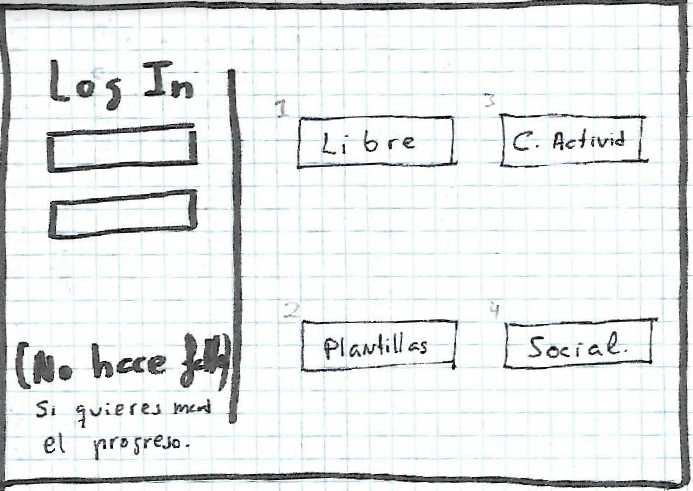
\includegraphics[width=0.7\linewidth]{Imagenes/Bitmap/logInAlfonso}
	\caption{Boceto de pantalla inicial}
	\label{fig:loginalfonso}
\end{figure}

Las Plantillas permitirían crear un tablero mediante el uso de una plantilla que cuenta con espacios donde colocar pictogramas. Las plantillas facilitan la creación del material que sigue una misma estructura, pero con contenido diferente. Un ejemplo de ello es la creación de un horario, donde pueden haber decenas de huecos a rellenar y se estructuran generalmente de la misma manera. Al tener una plantilla, el usuario se puede despreocupar de que los elementos queden bien centrados o añadir los días de la semana. En la Figura \ref{fig:inicioalfonso} podemos ver un ejemplo de algunas ideas de plantillas disponibles. 
La sección de Social tendría la función de compartir tableros, actividades y plantillas con la comunidad de usuarios.

% TODO: \usepackage{graphicx} required
\begin{figure}[h!]
	\centering
	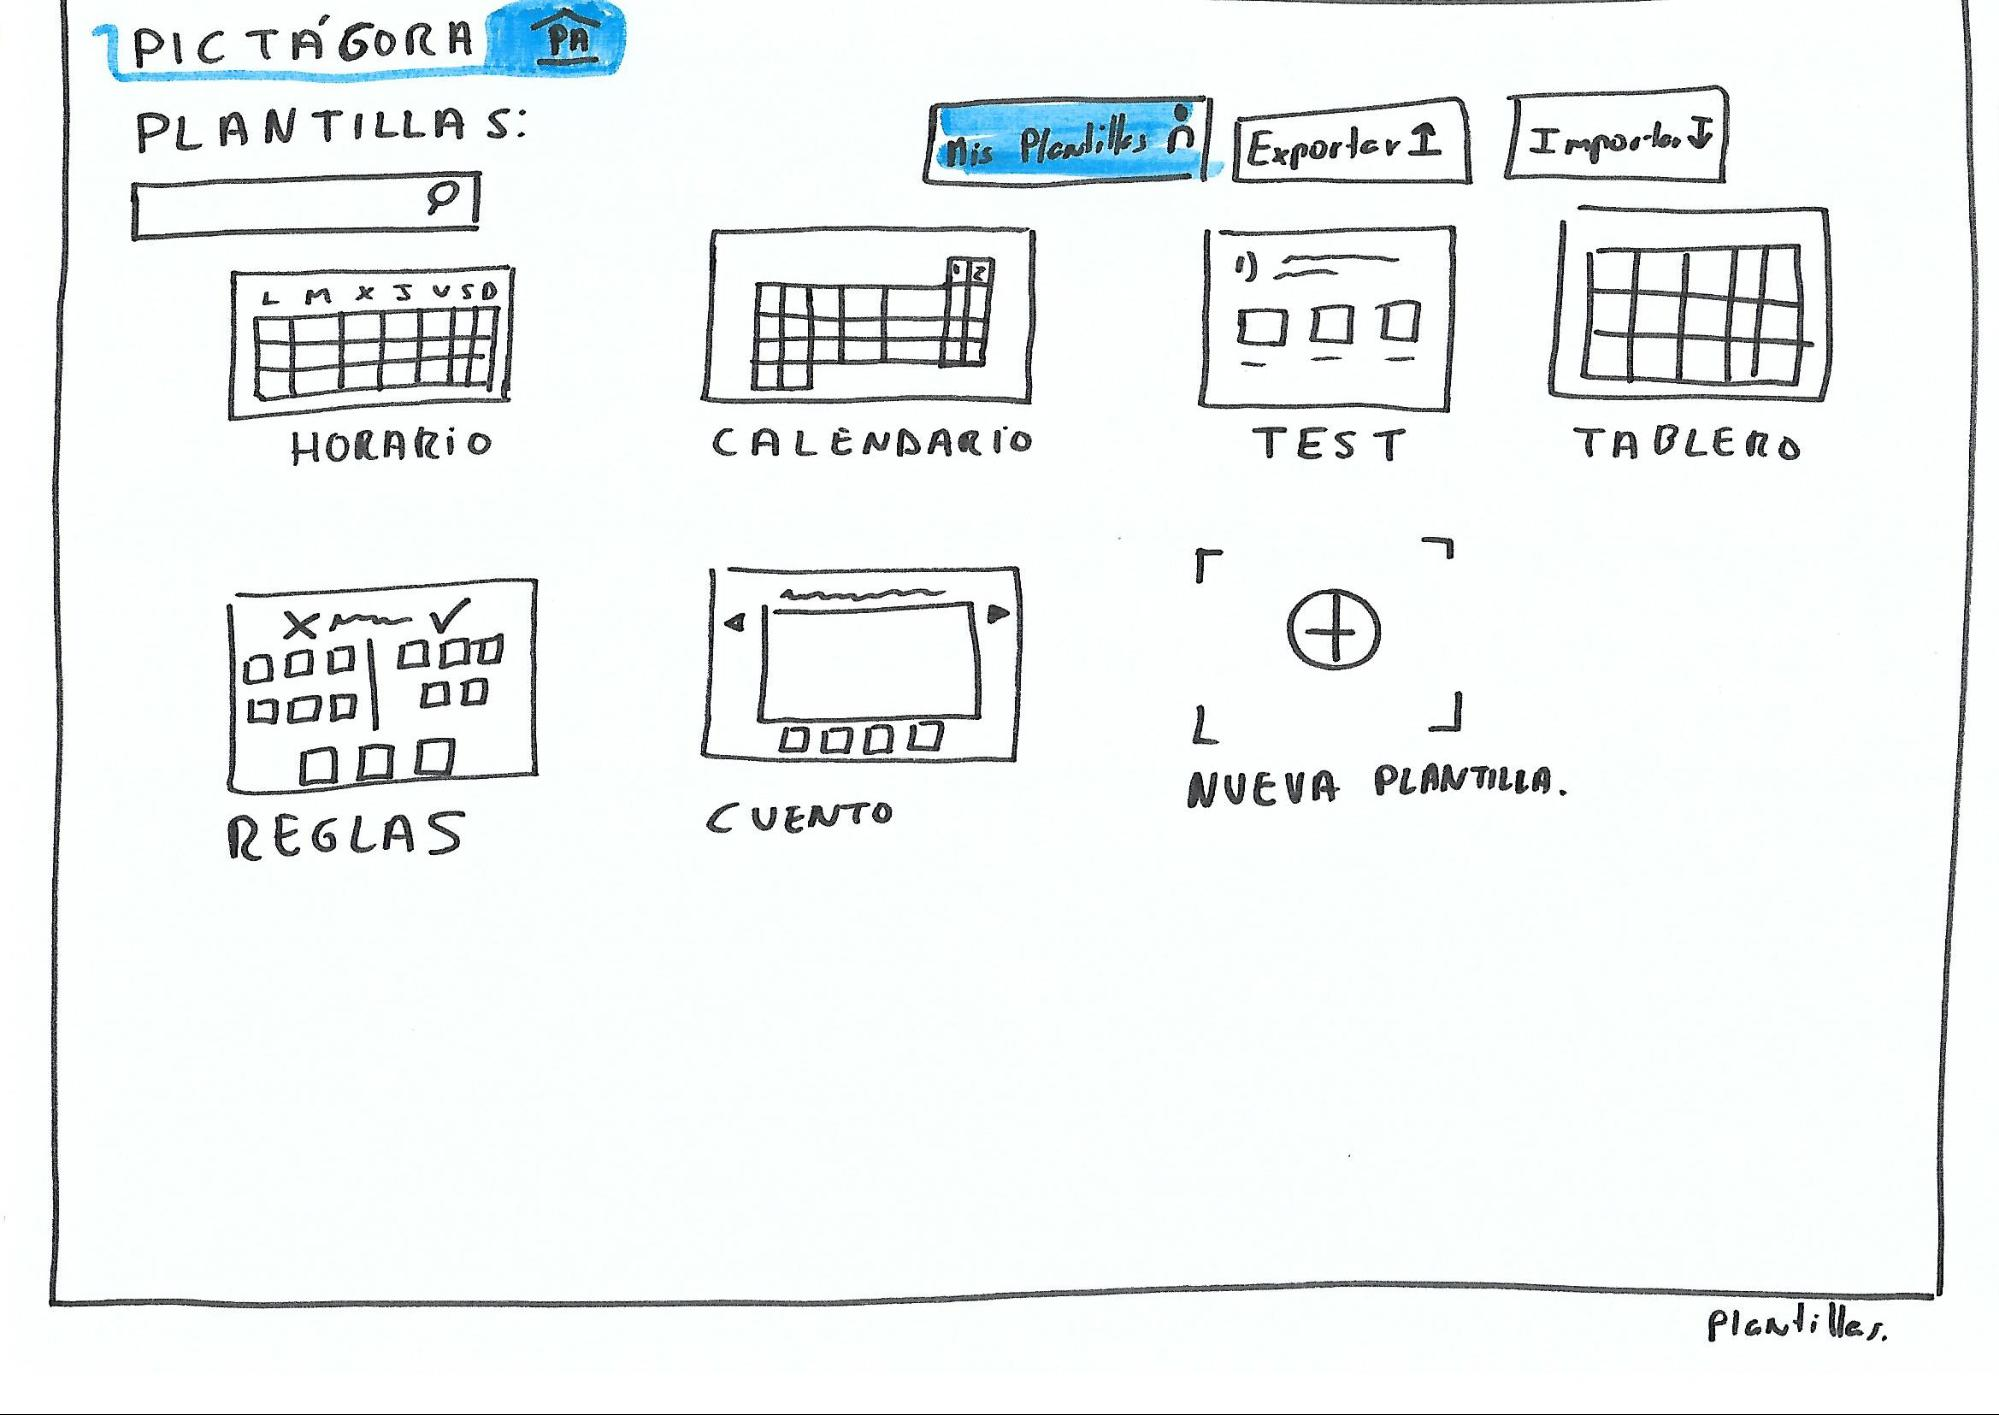
\includegraphics[width=0.7\linewidth]{Imagenes/Bitmap/inicioAlfonso}
	\caption{Boceto pantalla de plantillas}
	\label{fig:inicioalfonso}
\end{figure}


Por último, existe un inicio de sesión opcional para mantener el progreso entre dispositivos. Si profundizamos en la creación de un tablero en la Figura \ref{fig:dibujolibrealfon}, podemos ver los componentes que se pueden colocar sobre el tablero. Éstos son los pictogramas, texto, figuras como flechas o rectángulos y la posibilidad de subir imágenes. También comenzamos a plantear la idea de almacenar colecciones de pictogramas, que almacenan distintos conjuntos de pictogramas que el usuario agrupa según su criterio. Por ejemplo, si un profesor tiene que crear varios tableros respecto a un tema, como “Animales de la granja”, puede ser útil tener una colección con los pictogramas de gallina, cabra, oveja, etc. Agilizando el proceso de creación.

% TODO: \usepackage{graphicx} required
\begin{figure}[h!]
	\centering
	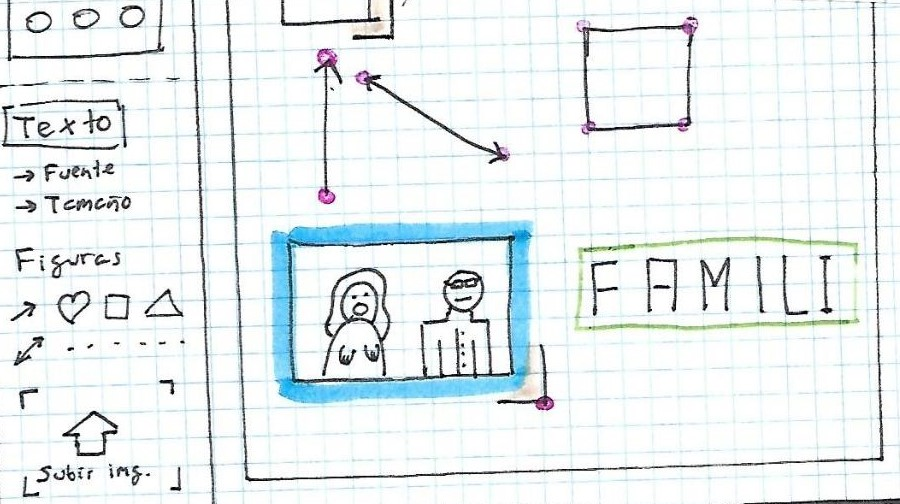
\includegraphics[width=0.7\linewidth]{Imagenes/Bitmap/DibujoLibreAlfon}
	\caption{Boceto pantalla de edición de tableros }
	\label{fig:dibujolibrealfon}
\end{figure}

El apartado de  creación de actividad no deja de ser una extensión de creación libre pero con más  componentes que permiten interacción con el usuario para crear distintos tipos de actividad. Estos componentes, que a partir de ahora denominaremos como \textbf{componentes interactivos} son:

\begin{itemize}
	
	\item \textbf{Cajón de pictgramas y espacio picto}: Se trata de dos componentes que van ligados entre sí. En primer lugar está el \textit{cajón de picto}, que es un espacio al margen del tablero donde aparecen un conjunto de pictogramas, como se puede ver en la Figura \ref{fig:componentecajon}. Los elementos que aparecen en el cajón pueden  ser desplazados a un \textit{espacio picto}. Esta componente es un hueco inicialmente vacío donde puede ser colocado un pictograma como se puede ver también en la Figura \ref{fig:componentecajon}. Ambos componentes son configurables, lo que permite establecer los pictogramas que aparecen en el \textit{cajón de pictogramas}, y los pictogramas que acepta el \textit{espacio picto}. Ambos elementos se beneficiarían de las colecciones, pues son conjuntos de pictogramas establecidos por el usuario.
	
	% TODO: \usepackage{graphicx} required
	\begin{figure}[h!]
		\centering
		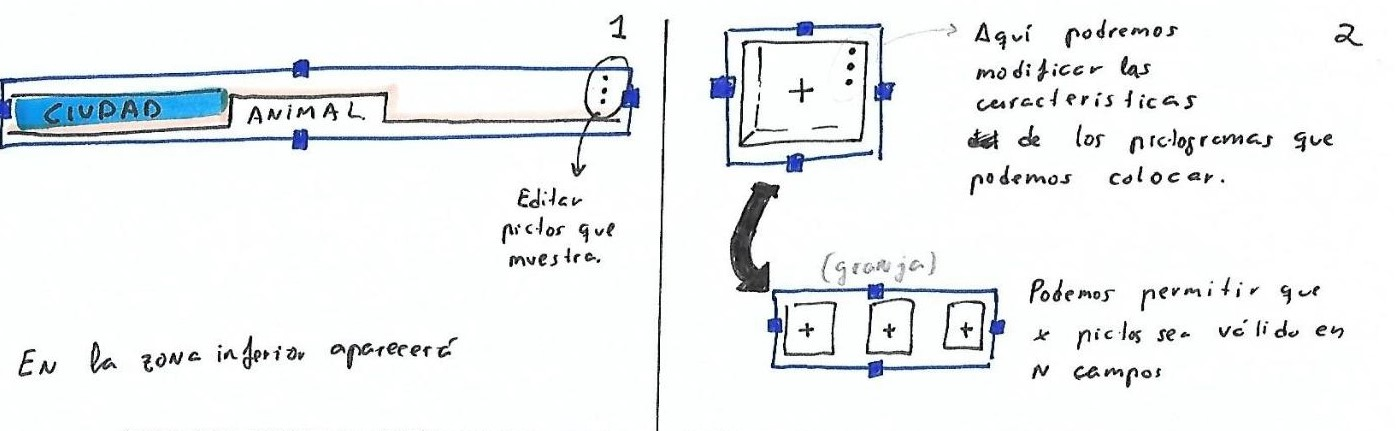
\includegraphics[width=0.7\linewidth]{Imagenes/Bitmap/componenteCajon}
		\caption{Boceto de las componentes canjón de picto y espacio picto.}
		\label{fig:componentecajon}
	\end{figure}
	
	
	Por ejemplo, un \textbf{cajón de pictgramas} podría tener asignado varias colecciones de pictogramas para que aparezcan mezclados. Asimismo, en el \textit{espacio picto} podría ser configurado para únicamente aceptar pictogramas de una de las colecciones o un pictograma concreto. De esta manera podría ser construido con facilidad un ejercicio donde el usuario que interactúe con el tablero pueda arrastrar distintos pictogramas del cajón de pictos a un espacio picto. En la Figura \ref{fig:cajonpictosgranja} se ve el \textit{cajón de pictos} mostrando pictogramas que representan animales de la granja y la selva, junto a unos \textit{espacio pictos} donde colocar los pictos de cada tipo.  El objetivo es dar la máxima flexibilidad al usuario que cree una actividad.
	
	
	% TODO: \usepackage{graphicx} required
	\begin{figure}[h!]
		\centering
		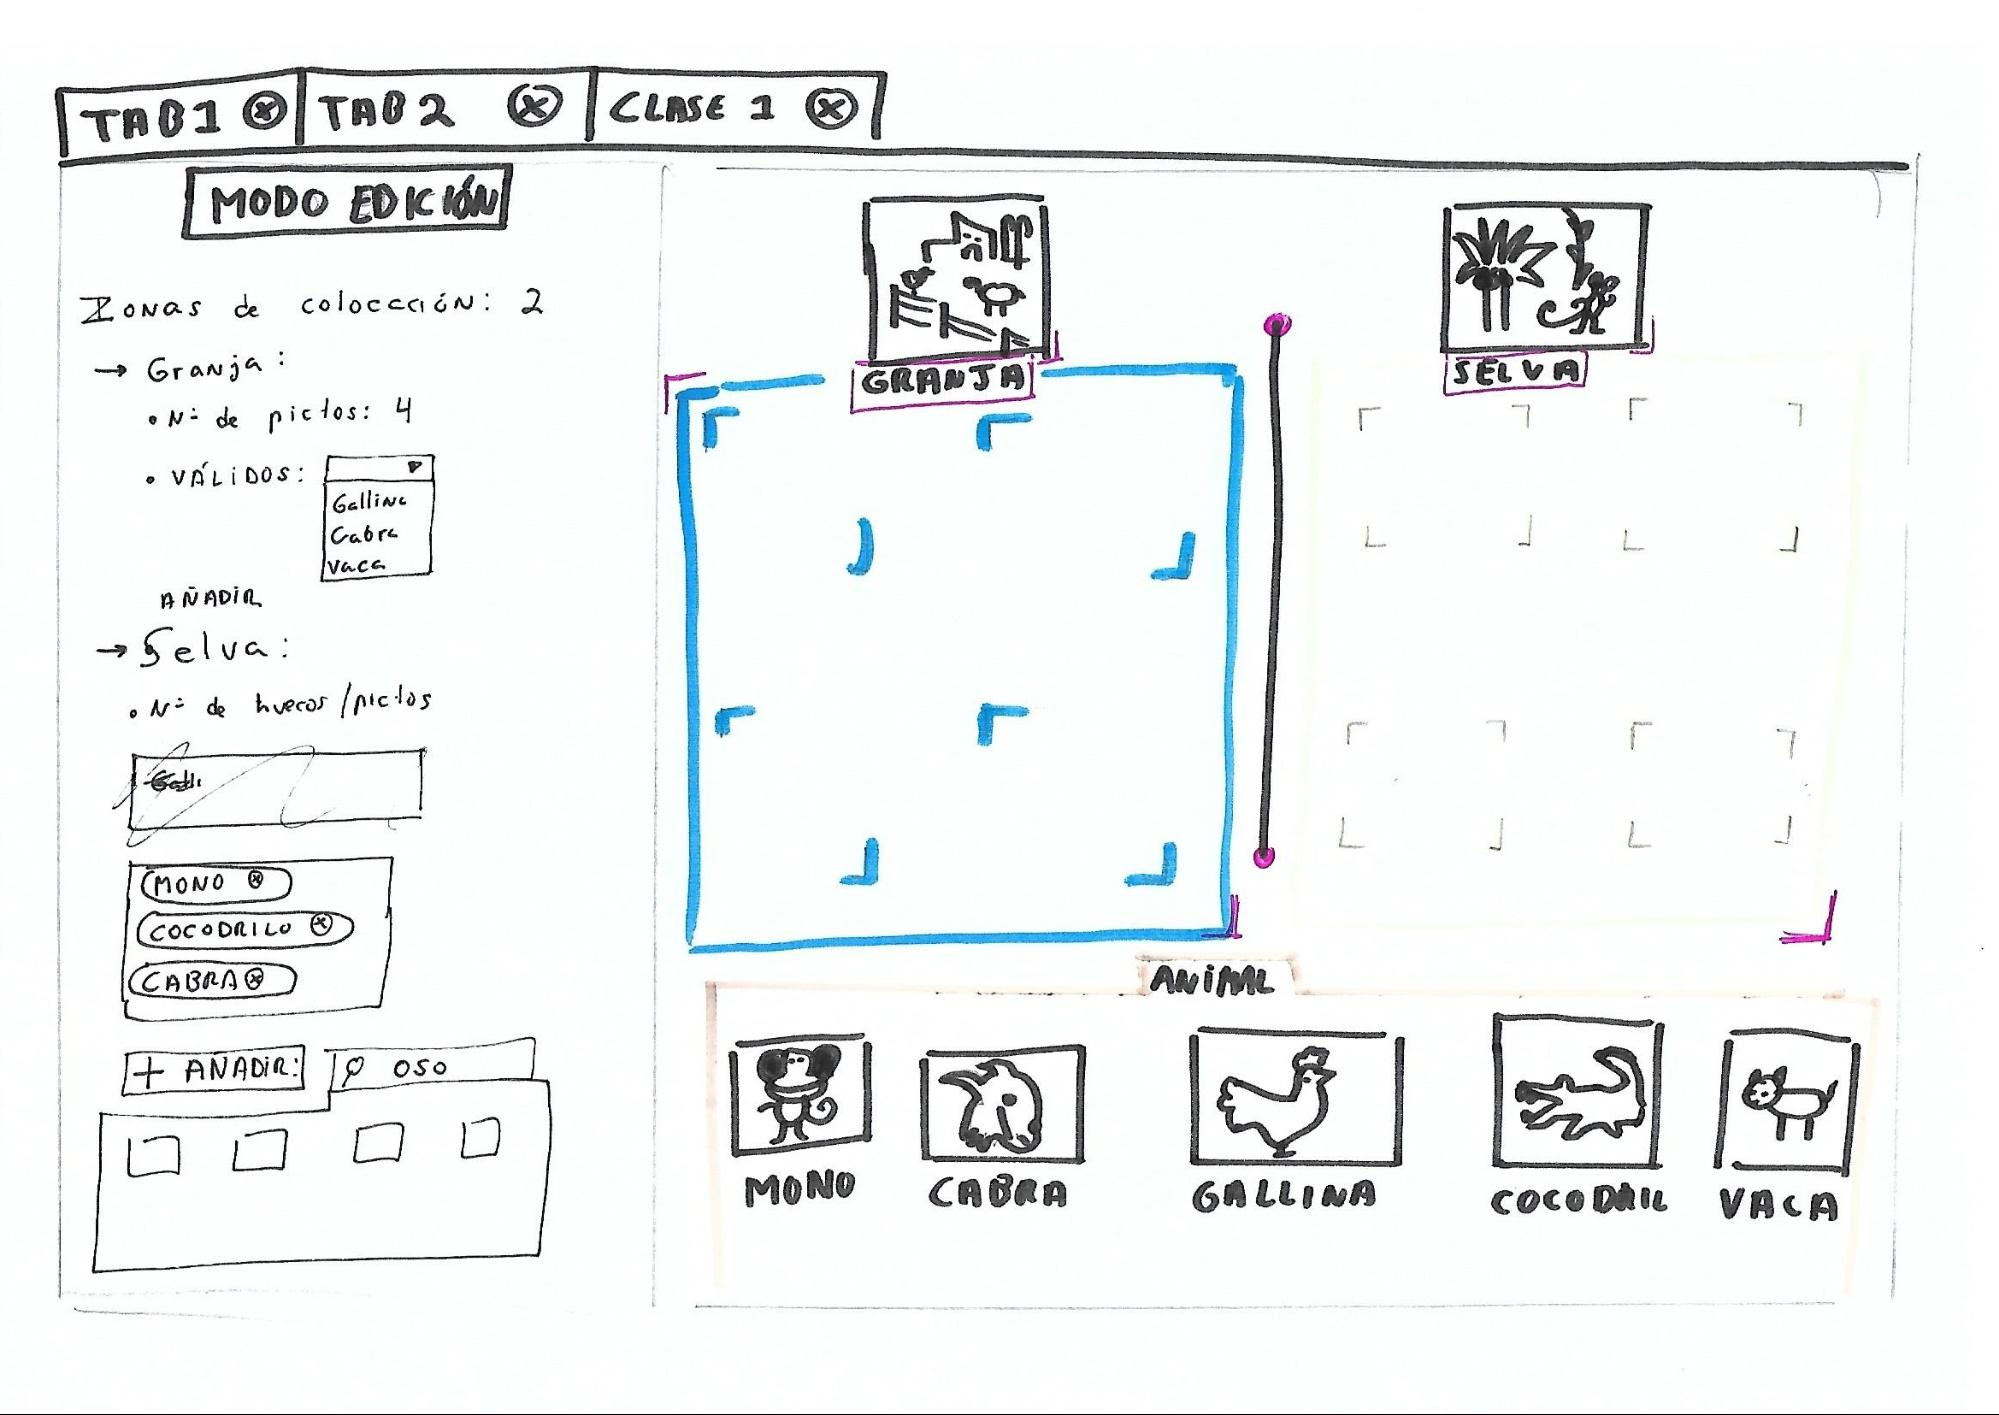
\includegraphics[width=0.9\linewidth]{Imagenes/Bitmap/cajonPictosGranja}
		\caption{Boceto de actividad con cajón de pictos y hueco picto}
		\label{fig:cajonpictosgranja}
	\end{figure}

	\item \textbf{Subtablero}: El componente subtablero permite desplegar un tablero de pictogramas. Los pictogramas que componen dicho tablero pueden venir dados por una colección de pictogramas creada por el usuario o indicarse en el propio componente. Su finalidad es la de añadir más pictogramas en el mismo espacio y agilizar la comunicación. La idea ha sido rescatada de Piktoplus \ref{cap2:pkplus} que también permitía crear subtableros.
	
	\item \textbf{Enlace}: Permite ligar dos pictogramas diferentes. Está compuesto por dos “piezas” las cuales se asignan a dos pictogramas para ser enlazados. Su finalidad es la de crear actividades como “hacer parejas”.
	
	En la Figura \ref{fig:componenteenla} podemos ver el ejemplo del pictograma hueso y perro, a los cuales se les asignan la misma pieza identificada por un símbolo de pica con fondo verde. El motivo por el que  las piezas tienen una forma y color asociado facilita al usuario que cree la actividad identificar las piezas ya  ligadas. El usuario final al pulsar sobre los pictos permitirá hacer parejas ,y completar la actividad.
	
	% TODO: \usepackage{graphicx} required
	\begin{figure}[h!]
		\centering
		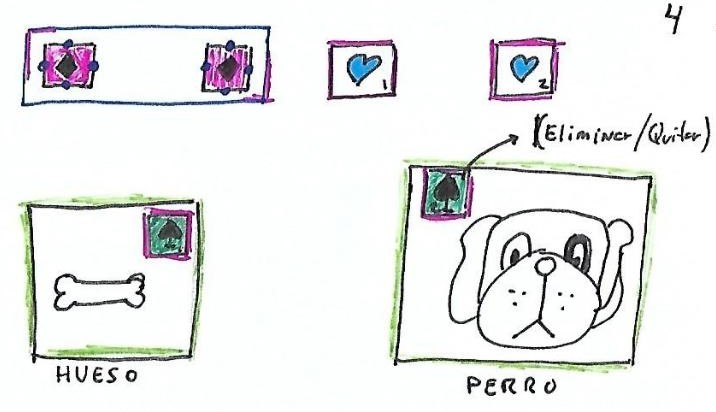
\includegraphics[width=0.7\linewidth]{Imagenes/Bitmap/componenteEnla}
		\caption{Boceto de las piezas que enlazan dos pictogramas al compartir la misma figura}
		\label{fig:componenteenla}
	\end{figure}

	
\end{itemize}

Con todos los tableros creados también es posible crear una actividad de mayor mediante la secuenciación de tableros. Se podría pasar de uno a las siguientes escenas mediante flechas, como se puede ver en la Figura \ref{fig:cuento}, que está compuesta por una fotografía y algunos pictogramas que la describen. Pero también se podrían intercalar estos tableros con otros que aporten interacción. Por ejemplo podría añadirse un test mediante el cajón de pictos para comprobar si se está comprendiendo la lectura.

% TODO: \usepackage{graphicx} required
\begin{figure}[h!]
	\centering
	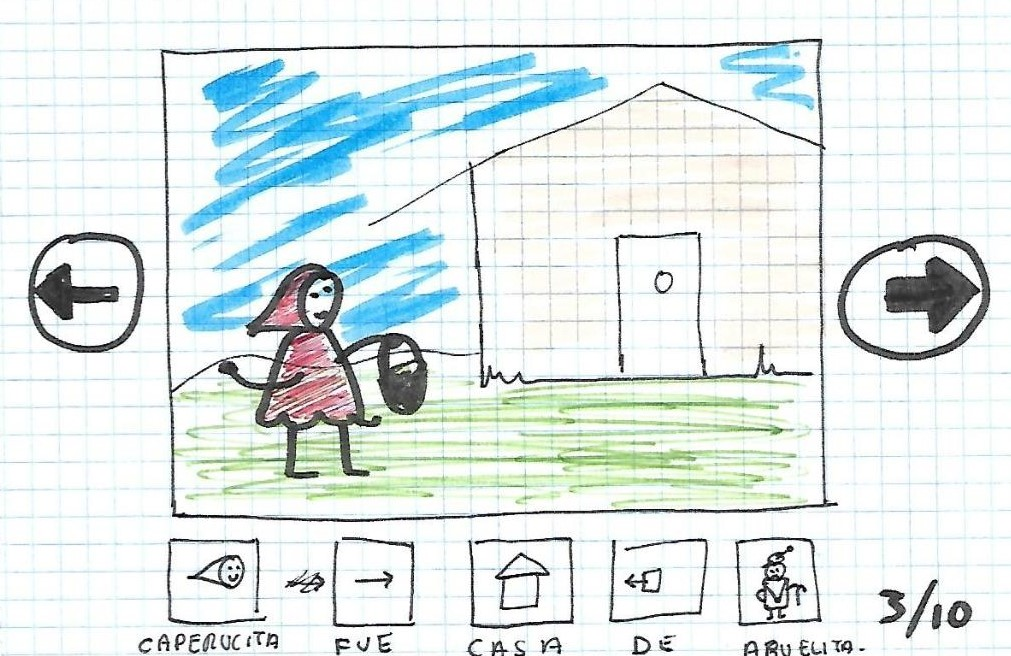
\includegraphics[width=0.7\linewidth]{Imagenes/Bitmap/Cuento}
	\caption{Boceto de una escena de un cuanto, con pictogramas en la zona inferior y botones en los laterales para pasar o retroceder la escena o tablero}
	\label{fig:cuento}
\end{figure}


En la Figura \ref{fig:presentaciontableros} podemos ver cómo se compondrían este tipo de actividades, que resulta muy familiar a la construcción de una presentación de diapositivas.  

% TODO: \usepackage{graphicx} required
\begin{figure}[h!]
	\centering
	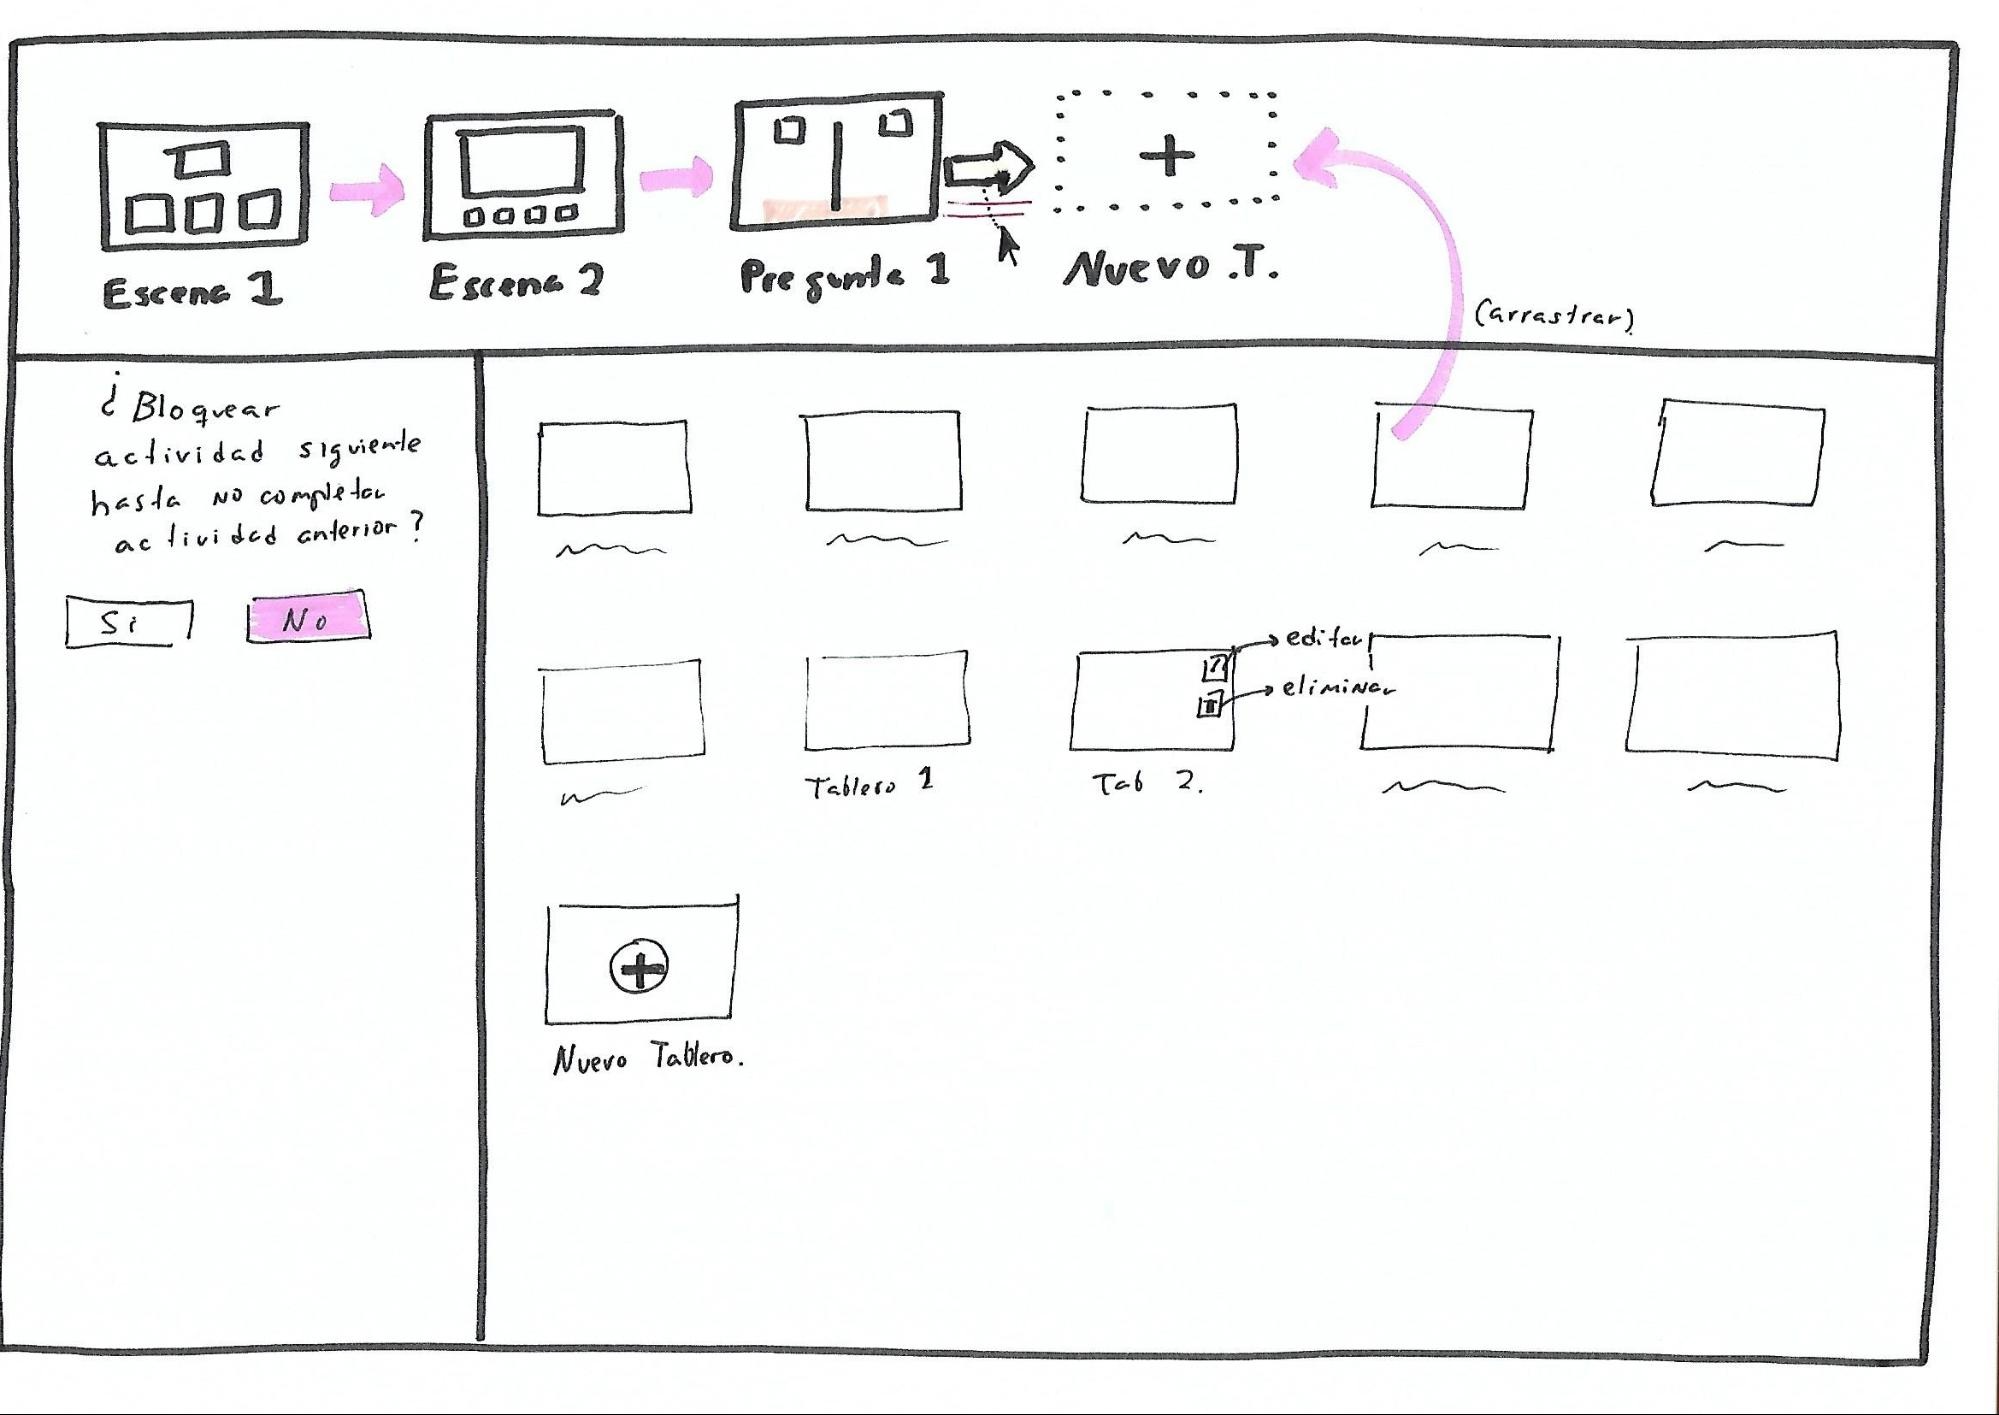
\includegraphics[width=0.7\linewidth]{Imagenes/Bitmap/presentacionTableros}
	\caption{Boceto del compositor de actividades}
	\label{fig:presentaciontableros}
\end{figure}


\subsection{Prototipo realizado por Jorge}

\begin{itemize}
	\item \textbf{Pantalla de inicio}
	
	En la Figura \ref{fig:iniciojorge} podemos ver la pantalla principal que nos encontraríamos al entrar a la aplicación. Podemos distinguir 4 botones que cada uno de ellos nos llevaría a su respectiva pantalla. 
	Tambíen podemos ver que en la parte superior de la pantalla tendríamos el nombre de la aplicación a la izquierda, que al pulsarlo volveríamos a esta pantalla, y un selector de idioma en la parte de la derecha. Esta parte sería común en las distintas pantallas de la aplicación.
	
	
% TODO: \usepackage{graphicx} required
\begin{figure}[h!]
	\centering
	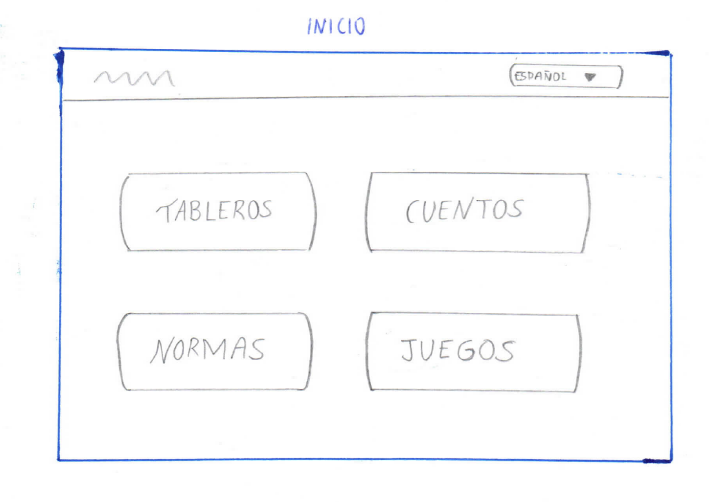
\includegraphics[width=0.7\linewidth]{Imagenes/Bitmap/inicioJorge}
	\caption{Pantalla de inicio con botones que muestran las otras pantallas de la aplicación.}
	\label{fig:iniciojorge}
\end{figure}

	
	\item \textbf{Pantalla del tablero}
	
	En la Figura \ref{fig:tablerosjorge} podemos ver pantalla de los tableros. En ella podríamos diferenciar claramente dos zonas, la parte de la izquierda correspondiente a la personalización del tablero y la parte de la derecha donde se mostraría el tablero que se está editando.
	
	
	En la parte de personalización del tablero podemos ver dos recuadros que englobarían diferentes posibilidades. Las funcionalidades que encontraríamos en el primer recuadro serían las siguientes:
	
	\begin{itemize}
		\item \textbf{Traducir frase}: dada una frase, mostraría toda la secuencia de pictogramas que tuviera ese significado. El botón de insertar que vemos insertaría toda la secuencia de pictogramas en el tablero.
		
		\item \textbf{Búsqueda simple de un pictograma}: dada una palabra concreta mostraría todos los pictogramas que tuvieran ese significado. Al igual que en el apartado anterior también tendríamos un botón de insertar el pictograma deseado al tablero.
	
	\end{itemize}

En el segundo recuadro tendríamos las siguientes opciones:

	\begin{itemize}
	
		\item \textbf{Insertar iconos}: al pulsarlo mostraría un modal con todos los iconos que se pueden añadir al tablero, al pulsar sobre uno de ellos se añadiría al tablero.
		
		\item \textbf{Insertar figuras geométricas}: al igual que con la funcionalidad anterior, al pulsarlo se abriría un modal donde se podrían seleccionar diferentes figuras geométricas para añadirlas al tablero.
		
		\item \textbf{Insertar imágenes}: esta herramienta permitiría al usuario insertar una fotografía que tuviera en su ordenador y a la hora de insertarla en el tablero tuviera las mismas propiedades que un pictograma, la imagen y un texto descriptivo.
		
		\item \textbf{Insertar un campo de texto}: permite añadir un campo en el tablero donde poner textos.
		
		\item \textbf{Editar el tamaño de letra del campo de texto}: esta funcionalidad solo estará disponible si hemos seleccionado un campo de texto en el tablero. Nos permite ajustar el tamaño del texto de un campo específico.
		
		\item \textbf{Editar la fuente del campo de texto}: al igual que con la funcionalidad anterior, deberemos seleccionar qué campo queremos editar. Permite cambiar la fuente del texto por otra.
		
	\end{itemize}
	
	
	En la zona inferior izquierda hay dos botones que permitirían guardar el estado de la página y volver a cargar el estado para posteriormente seguir trabajando con nuestro proyecto.
	
	En la parte superior tendríamos un botón llamado “\textit{Guardar como pdf}” que generaría un archivo con extensión pdf a partir del tablero inferior.
	
	
	En la zona de la derecha encontramos un tablero donde se insertaría todos los pictogramas, iconos, formas, imágenes y campos de texto. Todos los elementos que se inserten en el tablero podrán ser ampliados de tamaño pulsando sobre una de las esquinas del elemento.
	
	
	Debajo de dicho tablero encontramos un botón que nos permitiría añadir un nuevo tablero con el que seguir trabajando.
	
	
	
	% TODO: \usepackage{graphicx} required
	\begin{figure}[h!]
		\centering
		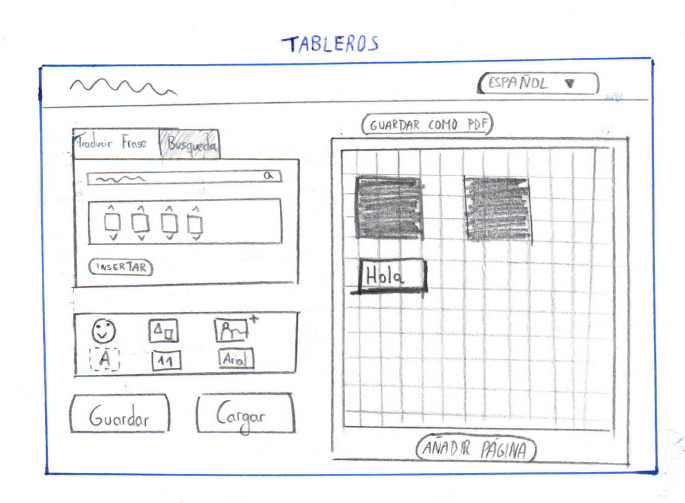
\includegraphics[width=0.7\linewidth]{Imagenes/Bitmap/tablerosJorge}
		\caption{Pantalla de configuración de tablero.}
		\label{fig:tablerosjorge}
	\end{figure}
	
	
	\item \textbf{Pantalla de normas y cuentos}
	
	En la Figura \ref{fig:normasjorge} al igual que en la pantalla del tablero distinguimos dos zonas, la parte de la izquierda perteneciente a la edición y la parte de la derecha donde veríamos el visionado de las normas o el cuento.
	
	% TODO: \usepackage{graphicx} required
	\begin{figure}[h!]
		\centering
		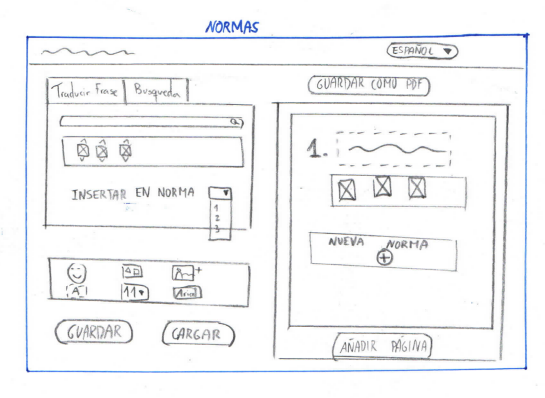
\includegraphics[width=0.7\linewidth]{Imagenes/Bitmap/normasJorge}
		\caption{Pantalla de configuración de normas.}
		\label{fig:normasjorge}
	\end{figure}
	
	También tenemos la posibilidad de guardar como pdf lo que tenemos en el tablero.
	
	
	La parte de la derecha sería distinta respecto a la pantalla de tableros ya que aquí el tablero no está cuadriculado. Para añadir una norma o una nueva sección en nuestro tablero tendríamos que pulsar sobre el botón “\textit{Nueva norma}” o “\textit{Nueva sección}” y se añadirían dos campos. El primero de ellos estaría numerado y en él se insertaría el texto correspondiente a la norma o a la sección del cuento. El segundo sería un campo en donde poder insertar los pictogramas que queramos que hicieran alusión al campo de texto superior. Además hay  un botón para añadir un nuevo tablero y seguir trabajando.
	
	
	\item \textbf{Pantalla de juegos}
	
	Para el apartado de juegos hay que distinguir dos pantallas, la primera de ellas sería la configuración del juego y la segunda sería la pantalla del juego.
	
	\begin{itemize}
		\item \textbf{Pantalla de configuración del juego}
		
		Al igual que en las pantallas anteriores la parte de la izquierda, ver la Figura \ref{fig:juegosjorge}, es la que se utilizará de cara a la edición del tablero para buscar  y añadir pictogramas, imágenes, iconos, etc.
		
		% TODO: \usepackage{graphicx} required
		\begin{figure}[h!]
			\centering
			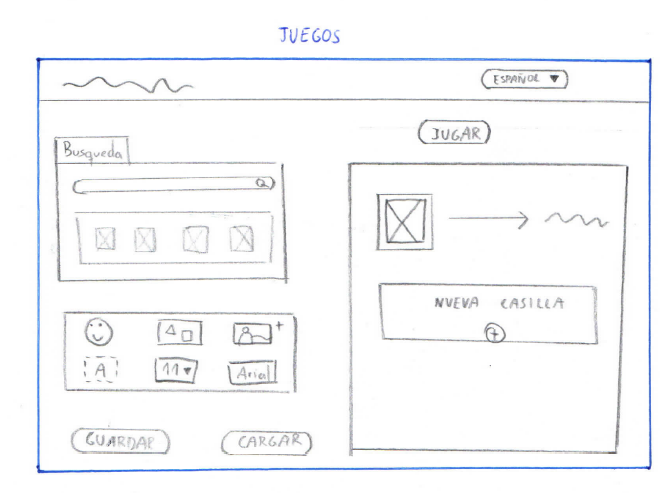
\includegraphics[width=0.7\linewidth]{Imagenes/Bitmap/juegosJorge}
			\caption{Pantalla de configuración de juego.}
			\label{fig:juegosjorge}
		\end{figure}
		
		También encontramos dos botones para guardar el estado de la configuración del juego y otro para cargar dicho estado y reanudar el trabajo realizado.
		
		
		Las funcionalidades que podemos encontrar en la parte del tablero son las siguientes:
		
		\begin{itemize}
			\item \textbf{Añadir una nueva casilla}: al pulsar sobre este botón se añadirá sobre el tablero sin cuadricular una casilla para insertar un pictograma, imagen, icono o figura geométrica, una flecha y un campo de texto.
			Esto permitirá crear una asociación entre un pictograma y su texto correspondiente para posteriormente ejecutar el juego.
			
			\item \textbf{Jugar}: en la parte superior tendremos un botón que al pulsarlo ejecutará el juego con las normas que estén creadas. Este botón al pulsarlo nos llevará a la pantalla de juego, ver Figura \ref{fig:juegojorge}.
			
		\end{itemize}
		
		\item \textbf{Pantalla de ejecución del juego}
		
		En esta pantalla, ver la Figura \ref{fig:juegojorge},  podremos ver todos los pictogramas que se han seleccionado en la pantalla de configuración y los textos asociados a cada uno de ellos.
		
		Todos los pictogramas seleccionados aparecerán en el recuadro superior de la pantalla. Estos pictogramas se podrán seleccionar y arrastrar a la casilla correspondiente de dicho pictograma.
		
		Si al arrastrar un pictograma y soltarlo en una casilla coincide con la norma definida por el usuario la fecha que une la casilla del pictograma y el texto se pondrá en verde indicando que es correcta esa relación. En caso de que no corresponda el pictograma con el texto, el pictograma volverá a la parte superior donde se encuentran todos los pictogramas indicando de esta manera que la asociación entre el pictograma y el texto no es la correcta.
		
		% TODO: \usepackage{graphicx} required
		\begin{figure}[h!]
			\centering
			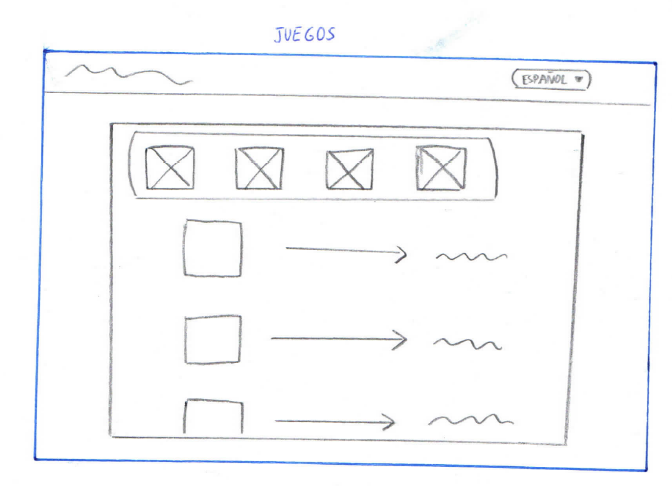
\includegraphics[width=0.7\linewidth]{Imagenes/Bitmap/juegoJorge}
			\caption{Pantalla de juego en ejecución.}
			\label{fig:juegojorge}
		\end{figure}
		
	\end{itemize}
	
\end{itemize}

\section{Requisitos de la aplicación}

\subsection{Herramientas}

En este apartado se incluirán todas aquellas funcionalidades que ayuden a la edición del tablero. Una de estas herramientas es la \textbf{búsqueda de pictogramas}, esta herramienta permitirá al usuario realizar una búsqueda a partir de una palabra e incluir el pictograma deseado en el tablero. También estará disponible la \textbf{herramienta de traducción de una frase} para facilitar al usuario la elaboración del tablero.

\begin{itemize}
	\item \textbf{Colecciones}: la herramienta colecciones ofrecen al usuario la opción de poder tener varias agrupaciones de los pictogramas que desee, según su conveniencia. Éstas están compuestas por un nombre que lo identifique y uno o varios pictogramas que el usuario elija según su criterio.
	
	\item \textbf{Importar y exportar}: estas herramientas ayudarán al usuario a poder guardar el estado de la página y poder editarlo posteriormente. 
\end{itemize}


\subsection{Componentes}


En esta sección desarrollaremos los principales componentes que pueden colocarse sobre el tablero. 

Un componente es \textbf{un elemento que puede ser añadido al tablero} e incluso añadir interacción para al usuario final. Distinguiremos dos tipos de componentes, los \textbf{básicos} que no añaden ninguna interacción y los \textbf{componentes interactivos}, que pueden ser modificados y añadir comportamientos específicos al usuario final.

\begin{itemize}
	
	
	\item \textbf{Picto}: El elemento picto representa un pictograma junto a su nombre asociado. Cuenta con la opción de poder modificar algunas características del pictograma, como indicar un tiempo verbal, el plural. Si el pictograma muestra a una persona, también se puede cambiar el color de pelo y tono de piel.
	
	\item \textbf{Foto}: El elemento foto, permite añadir imágenes tanto a partir de una URL como las que suba el propio usuario. Esta ha sido una de las características más demandadas por los usuarios. Al permitir añadir fotos abre multitud de posibilidades, como la de poner fotos de la familia, mostrar localizaciones habituales como la cocina e identificar objetos personales que no se representan tan fielmente mediante un pictograma (Por ejemplo, un juguete específico o la portada de su  libro favorito). Esto facilita al usuario final relacionar conceptos al mostrar figuras que le sean familiares.
	
	\item \textbf{Figuras}: Las figuras, sirven para ordenar, enfatizar o decorar el tablero. Un ejemplo, sería una línea que puede ser usada para dividir el espacio de trabajo en secciones, relacionar dos pictogramas o incluso marcar un espacio donde escribir una respuesta si se va a imprimir el tablero. Pese a la simplicidad de las figuras, sus posibilidades son muy amplias, según  la creatividad de quien cree el tablero.
	
	\item \textbf{Campos de texto}: Los campos de texto podrán ser insertados en el tablero de la aplicación. Estos campos de texto podrán ser editados permitiendo cambiar el color del texto y aumentar la fuente.
	
	\item \textbf{Cajón de Pictogramas}: El cajón de pictos es un apartado al margen del tablero donde aparecen un conjunto de pictogramas que el usuario debe mover a alguna posición. En el hueco donde vayan los pictogramas que se encuentren en el cajón de pictogramas puede ser modificado y aceptar unos u otros. Esto puede ser utilizado como test sencillo de hacer y usar.
	
	\item \textbf{Subtablero}: El Subtablero es un componente que a simple vista parece un pictograma pero al ser pulsado, despliega un tablero que contiene otros pictogramas. Este concepto la ha sido rescatada de Piktoplus, la cual actualmente no cuenta con soporte y puede ser de utilidad para añadir más pictogramas en el mismo espacio.
\end{itemize}

Respecto a los elementos \textbf{descartados}, a continuación se detallarán los elementos que fueron descartados y sus motivos:

\begin{itemize}
	\item\textbf{Pantallas de normas y cuentos predefinidos}: El principal motivo es su falta de flexibilidad, es decir que si la aplicación no permite crear un cuento o un listado de reglas con sus propias herramientas, tampoco permitirá crear otro tipo de material. Por ello se ha decantado por herramientas que ofrecieran más posibilidades al usuario. Otro motivo era que no todos los usuarios querrían por ejemplo que las normas aparecen de una misma manera, como si fuese un listado. Por lo que es imprescindible ofrecer la mayor libertad posible al usuario.
	
	\item \textbf{Plantillas}: Tras comentarlo en las reuniones, no se centró mucha atención en este apartado, pues ya estaba muy explorado por la aplicación Pictableros.
	
	\item \textbf{Log In}: El principal motivo de su descarte, fue el no poder garantizar en un primer momento la total seguridad de los tableros creados.
	Otra de las características del proyecto es la inclusión de imágenes que pudiera subir el usuario, con la responsabilidad añadida de haber imágenes de menores de edad por medio. Estos fueron los motivos por los que optamos por una modalidad sin necesidad de servidor, donde los documentos generados se guardan en el ordenador.
	
	\item \textbf{Selección de idioma}: Fue una idea descartada al principio del desarrollo, en vista a que la gran mayoría de las aplicaciones existentes ofrecían soporte en multitud de idiomas. Pero no se llevó a cabo para centrarnos en otros aspectos con mayor relevancia.
	
\end{itemize}






